\PassOptionsToPackage{unicode=true}{hyperref} % options for packages loaded elsewhere
\PassOptionsToPackage{hyphens}{url}
%
\documentclass[man]{apa6}
\usepackage{lmodern}
\usepackage{amssymb,amsmath}
\usepackage{ifxetex,ifluatex}
\usepackage{fixltx2e} % provides \textsubscript
\ifnum 0\ifxetex 1\fi\ifluatex 1\fi=0 % if pdftex
  \usepackage[T1]{fontenc}
  \usepackage[utf8]{inputenc}
  \usepackage{textcomp} % provides euro and other symbols
\else % if luatex or xelatex
  \usepackage{unicode-math}
  \defaultfontfeatures{Ligatures=TeX,Scale=MatchLowercase}
\fi
% use upquote if available, for straight quotes in verbatim environments
\IfFileExists{upquote.sty}{\usepackage{upquote}}{}
% use microtype if available
\IfFileExists{microtype.sty}{%
\usepackage[]{microtype}
\UseMicrotypeSet[protrusion]{basicmath} % disable protrusion for tt fonts
}{}
\IfFileExists{parskip.sty}{%
\usepackage{parskip}
}{% else
\setlength{\parindent}{0pt}
\setlength{\parskip}{6pt plus 2pt minus 1pt}
}
\usepackage{hyperref}
\hypersetup{
            pdftitle={Carrying out Latent Profile Analysis in Accordance With Best Practices: A Tutorial Using the tidyLPA R package},
            pdfauthor={Joshua Rosenberg, Caspar van Lissa, Jennifer Schmidt, Patrick Beymer, Daniel Anderson, \& Matthew Schell},
            pdfkeywords={Latent Profile Analysis, mixture models, finite mixture models, tutorial, R, MPlus, mclust},
            pdfborder={0 0 0},
            breaklinks=true}
\urlstyle{same}  % don't use monospace font for urls
\usepackage{graphicx,grffile}
\makeatletter
\def\maxwidth{\ifdim\Gin@nat@width>\linewidth\linewidth\else\Gin@nat@width\fi}
\def\maxheight{\ifdim\Gin@nat@height>\textheight\textheight\else\Gin@nat@height\fi}
\makeatother
% Scale images if necessary, so that they will not overflow the page
% margins by default, and it is still possible to overwrite the defaults
% using explicit options in \includegraphics[width, height, ...]{}
\setkeys{Gin}{width=\maxwidth,height=\maxheight,keepaspectratio}
\setlength{\emergencystretch}{3em}  % prevent overfull lines
\providecommand{\tightlist}{%
  \setlength{\itemsep}{0pt}\setlength{\parskip}{0pt}}
\setcounter{secnumdepth}{0}
% Redefines (sub)paragraphs to behave more like sections
\ifx\paragraph\undefined\else
\let\oldparagraph\paragraph
\renewcommand{\paragraph}[1]{\oldparagraph{#1}\mbox{}}
\fi
\ifx\subparagraph\undefined\else
\let\oldsubparagraph\subparagraph
\renewcommand{\subparagraph}[1]{\oldsubparagraph{#1}\mbox{}}
\fi

% set default figure placement to htbp
\makeatletter
\def\fps@figure{htbp}
\makeatother

\usepackage{etoolbox}
\makeatletter
\providecommand{\subtitle}[1]{% add subtitle to \maketitle
  \apptocmd{\@title}{\par {\large #1 \par}}{}{}
}
\makeatother

\title{Carrying out Latent Profile Analysis in Accordance With Best Practices: A Tutorial Using the tidyLPA R package}
\author{Joshua Rosenberg\textsuperscript{1}, Caspar van Lissa\textsuperscript{2}, Jennifer Schmidt\textsuperscript{3}, Patrick Beymer\textsuperscript{3}, Daniel Anderson\textsuperscript{4}, \& Matthew Schell\textsuperscript{3}}
\date{}

\authornote{Add complete departmental affiliations for each author here. Each new line herein must be indented, like this line.

Enter author note here.

Correspondence concerning this article should be addressed to Joshua Rosenberg, 1122 Volunteer Blvd., Knoxville, TN, 37996. E-mail: \href{mailto:jmrosenberg@utk.edu}{\nolinkurl{jmrosenberg@utk.edu}}}

\abstract{

}

\begin{document}
\maketitle

\hypertarget{introduction}{%
\section{Introduction}\label{introduction}}

In statistics classes, textbooks, and workshops, an example like the following is common:

\begin{quote}
Grades are normally distributed, with \(\mu\) = 75, \(\sigma\) = 5.
\end{quote}

Students, may (reasonably) ask, though, are grades \emph{really} normally distributed?

Are their one distribution?

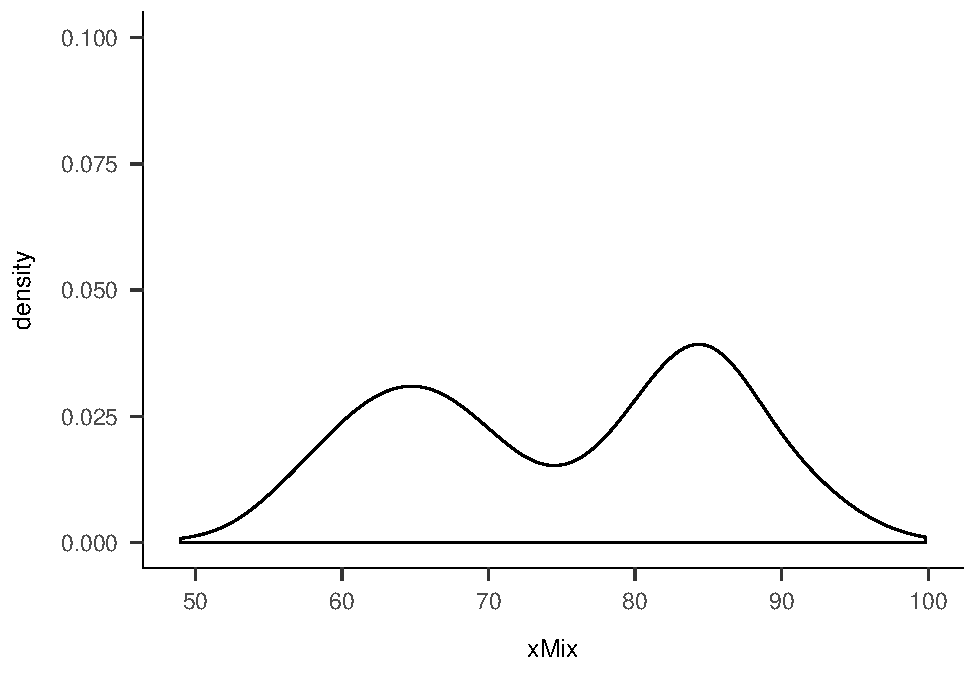
\includegraphics{paper_files/figure-latex/echo - FALSE-1.pdf}

Or two?

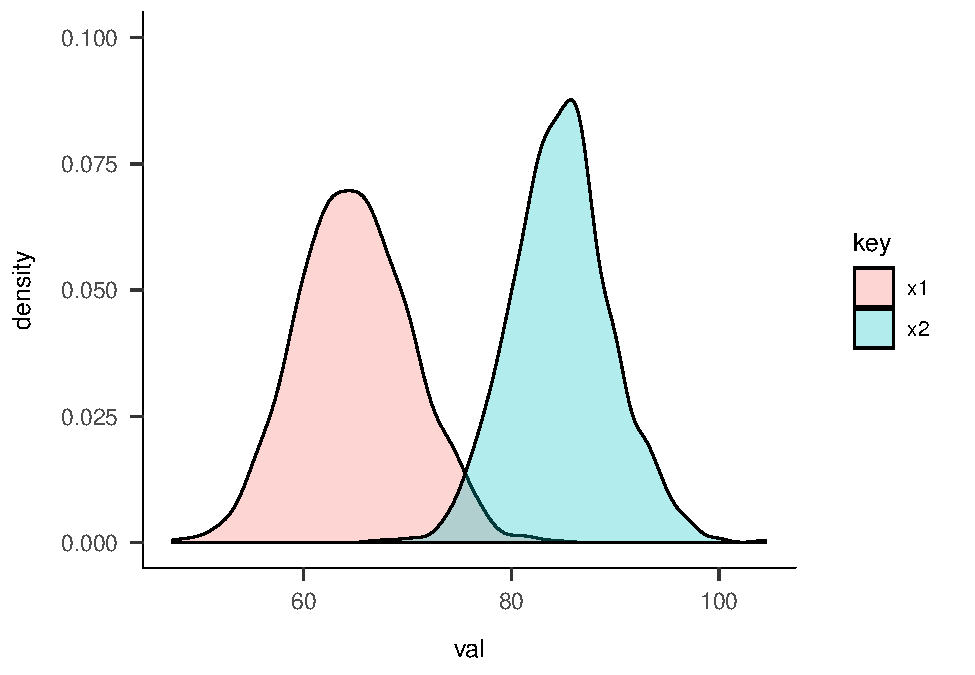
\includegraphics{paper_files/figure-latex/unnamed-chunk-2-1.pdf}

This kind of distribution (that is \emph{bimodal}) is not exclusive to grades. For
teachers, psychologists, researchers, and friends and family members, people are
highly-complex and not easily able to be characterized by \emph{one} characteristic
or personality trait--and its distribution. In the social sciences, broadly, and
in psychology, particularly, a statistical method that can be used to describe
how people, in their individual particularities, may have similarities on the
basis of some set of measures through which they can be grouped in meaningful,
distinctive ways. This approach, which has a provenance in developmental (or
\emph{person-oriented}) approaches (Bergman \& El-Khouri, 1997; Magnusson \&
Cairns, 1996; see Linnenbrink-Garcia \& Wormington, 2017, for a recent review) is
an example of a general mixture model (Harring \& Hodis, 2016; Pastor, Barron,
Miller, \& Davis, 2007).

In this tutorial, we aim to describe one of the most commonly-used--and relevant
to psychologists--application of the general mixture model, to cases for which
all of the variables for which (relatively) homogeneous groups are identified
from among a (relatively) heterogeneous sample are continuos, \emph{latent profile
analysis} (LPA). We note that scholars using the approach, especially in
developmental and educational psychology, use cluster analytic methods. Such an
approach has some similarities with LPA (CITE paper showing how k-means is
similar to the simplest model specification of LPA?), though LPA also has a
number of benefits (Linnenbrink-Garcia \& Wormington, 2017), and we we focus on
LPA in this paper.

After describing the method and some examples of its use, we provide a tutorial
for carrying out LPA in the context of a freely-available, open-source
statistical software package we created for R (R Core Team, 2019), tidyLPA.
Finally, we offer some ideas about best practices and informed recommendations
for researchers aiming to use LPA in their applied work, and conclude with
reflections on the role of statistical software--especially software that is
freely-available, open-source, and highly-performant--in the psychological
sciences.

\hypertarget{latent-profile-analysis}{%
\section{Latent Profile Analysis}\label{latent-profile-analysis}}

The goal of LPA is estimate the parameters for a number of distributions
(typically multivariate) from a single dataset. Thus, such an approach is
model-based, and some descriptions in the literature refer to it as model-based
clustering (Hennig, Meila, Murtagh, \& Rocci, 2015; Scrucca, Fop, Murphy, \&
Raftery, 2017). Thus, one distinction between LPA and other, similar cluster
analytic approaches is that LPA is model-based; instead of using algorithms to
group together cases, LPA seeks to estimate parameters - in terms of variances
and covariances and how they are the same or different across profiles - that
best characterize the different distributions. Then, this approach seeks to
assign to each observation a probability that the observation is a sample from
the population associated with each profile (or mixture component).

Because LPA is model-based, a number of different model parameterizations can be
estimated. These models differ in terms of whether--and how--parameters are
estimated across the profiles. These parameters are the means for the different
profiles, which, in this approach, always are estimated freely across the
profiles; the variances for the variables used to create the profiles, which can
be estimated freely or can be estimated to be the same, or equal, across
profiles; and the covariances of the variables used to create the profiles,
which can be freely-estimated, estimated to be equal, or fixed to be zero.

We wish to note that challenge facing the analyst using LPA is that these
parameters and the distinct model parameterizations that can be estimated is the
different terminology used. As one example, Scrucca et al. (2017) refer to these
parameterizations not in terms of whether and how parameters are estimated, but
rather in terms of the geometric properties of the distributions that result
from particular parameterizations. Muthen and Muthen (1997-2017) and others
(Pastor et al., 2007) commonly refer to local independence to mean that the
covariances are fixed to zero (also described as the specification of the
covariance matrix as ``diagonal,'' because only the diagonal components, or the
variances, are estimated).

In general, as more parameters are estimated (i.e., those that are fixed to zero
are estimated as being equal across profiles; or those estimated as being equal
across profiles are freely-estimated across them), the model becomes more
complex; the model may fit better, but also be overfit, meaning that the
profiles identified may be challenging to replicate with another, separate data
set. Even still, flexibility in terms of which models can be estimated also has
affordances. For example, the varying means, equal variances, and covariances
fixed to 0. A researcher might choose this model specification if she wants to
model the variables to be used to create profiles that are independent. This
model is very simple, as no covariances are estimated and the variances are
estimated to be the same across profiles. As we estimate more parameters (and
decrease the degrees of freedom), we are more likely to fit the data, but less
likely to be able to replicate the model with a second set of data. In other
words, more parameters may mean a loss of external validity. As we progress
toward more complex models (with increasingly complex parameterization), then we
are more likely to fit the data better. More information on the model
parameterizations are discussed in the context of the software tool tidyLPA that
we have developed.

A note of caution is warranted about LPA in the context of their characteristics
and strengths. Bauer (2007) notes that many samples of data can be usefully
broken down into profiles, and that the addition of profiles will likely be
suggested for reasons other than the samples coming from more than one
distribution (i.e., due to non-normality in the variables measured). Bauer also
cautions that profiles should not be reified; that profiles do not necessarily
exist outside of the analysis that they should be interpreted more as useful
interpretative devices. These cautions suggest that, in general, parsimony,
interpretability, and a general sense that the profiles are not necessarily
real, but are rather helpful analytic tools, should be both priorities for the
analyst and the reader of studies using this approach.

\hypertarget{specific-software-tools}{%
\section{Specific Software Tools}\label{specific-software-tools}}

\hypertarget{other-tools}{%
\subsection{Other Tools}\label{other-tools}}

SPSS is a common tool to carry out cluster analyses (but not LPA). While
somewhat straightforward to carry out, particularly in SPSS's graphical user
interface (GUI), there are some challenges to use of this approach. The GUI in
SPSS can be challenging, even for the most able analyst, to be able to document
every step with syntax, and so reproducing the entire analysis efficiently can
be a challenge, both for the analyst exploring various solutions and for the
reviewer looking to replicate this work. Additionally, SPSS is commercial
software (and is expensive), and so analysts access to it cannot carry out this
analysis.

Another common tool is MPlus (Muthen \& Muthen, 2019). MPlus is a commercial tool
that provides functionality for many latent variable (and multi-level) models.
We will speak more to MPlus in the section on tidyLPA, as our software provides
an interface to both it and an open-source tool.

In R, a number of tools \emph{can} be used to carry out LPA. OpenMx can be used for
this purpose (and to specify almost any model possible to specify within a
latent variable modeling approach). However, while OpenMx is very flexible, it
can also be challenging to use. Other tools in R allow for estimating Gaussian
mixture models, or models of multivariate Gaussian (or normal) distributions. In
addition to following the same general approach, using tools that are designed
for Gaussian mixture modeling have other benefits, some efficiency-related (see
RMixMod, which uses compiled C++ code) and others in terms of ease-of-use (i.e.,
the plot methods built-in to RMixMod, mclust, and other tools). However, they
also have some drawbacks, in that it can be difficult to translate between the
model specifications, which are often described in terms of the geometric
properties of the multivariate distributions being estimated (i.e., ``spherical,
equal volume''), rather than in terms of whether and how the means, variances,
and covariances are estimated. They also may use different default settings
(than those encountered in MPlus) in terms of the expectation-maximization
algorithm, which can make comparing results across tools challenging.

\hypertarget{tidylpa}{%
\subsection{tidyLPA}\label{tidylpa}}

Because of the limitations in other tools, we set out to develop a tool that a)
provided sensible defaults and were easy to use, but provided the option to
access and modify all of the inputs to the model (i.e., low barrier, high
ceiling), b) interfaced to existing tools, and are able to translate between
what existing tools are capable of and what researchers and analysts
carrying-out person-oriented analyses would like to specify, c) made it easy to
carry-out fully-reproducible analyses and d) were well-documented. To do so, we
created tidyLPA (Rosenberg, Beymer, Anderson, Lissa, \& Schmidt, 2018).

This package focuses on models that are commonly specified as part of LPA.
Because MPlus is so widely-used, it can be helpful to compare output from other
software to MPlus. The functions in tidyLPA that use mclust have been
benchmarked to MPlus for a series of simple models (with small datasets and for
models with small numbers of profiles. This R Markdown output contains
information on how mclust and Mplus compare. The R Markdown to generate the
output is also available here, and, as long as you have purchased MPlus (and
installed MplusAutomation), can be used to replicate all of the results for the
benchmark. Note that most of the output is identical, though there are some
differences in the hundreths decimal places for some. Because of differences in
settings for the EM algorithm and particularly for the start values (random
starts for MPlus and starting values from hierarchical clustering for mclust),
differences may be expected for more complex data and models.

One way that tidyLPA is designed to be easy to use is that it assumes a ``tidy''
data structure (Wickham, 2014). This means that it emphasizes the use of a data
frame as both the primary input and output of functions for the package. Because
data is passed to and returned (in amended form, i.e., with the latent profile
probabilities and classes appended to the data) from the function, it makes it
easy to create plots or use results in subsequent analyses. Another noteworthy
feature of tidyLPA is that it provides the same functionality through two
different tools, one that is open-source and available through R, the mclust
package (Scrucca et al., 2017) and one that is available through the commercial
software MPlus (Muthen \& Muthen, 1997-2017). Moreover, as both tools use the
same maximum likelihood estimation procedure, they are benchmarked to produce
the same output. Also, note that we have described the model
specifications with descriptions of what is estimated in terms of the variances
and covariances, the common names for the models (i.e., class-varying
unrestricted), and the covariance matrix associated with the parameterizationfor
the six models that are possible to be estimated on the website for tidyLPA (see
here).

\hypertarget{installation}{%
\subsection{Installation}\label{installation}}

You can install tidyLPA from CRAN with:

You can also install the development version of tidyLPA from GitHub with:

\hypertarget{examples}{%
\subsection{Examples}\label{examples}}

\hypertarget{mclust-via-tidylpa}{%
\subsubsection{Mclust via tidyLPA}\label{mclust-via-tidylpa}}

Here is a brief example using the built-in \texttt{pisaUSA15} data set and variables
for broad interest, enjoyment, and self-efficacy. Note that we first type the
name of the data frame, followed by the unquoted names of the variables used to
create the profiles. We also specify the number of profiles and the model. See
\texttt{?estimate\_profiles} for more details.

In these examples, we pass the results of one function to the next by \emph{piping}
(using the \texttt{\%\textgreater{}\%} operator, loaded from the \texttt{dplyr} package). We pass the data to
a function that selects relevant variables, and then to \texttt{estimate\_profiles}:

\begin{verbatim}
## tidyLPA analysis using mclust: 
## 
##  Model Classes AIC    BIC    Entropy prob_min prob_max n_min n_max BLRT_p
##  1     3       629.10 665.57 0.82    0.83     0.96     0.03  0.70  0.01
\end{verbatim}

\hypertarget{mplus-via-tidylpa}{%
\subsubsection{Mplus via tidyLPA}\label{mplus-via-tidylpa}}

We can use Mplus simply by changing the package argument for
\texttt{estimate\_profiles()}:

A simple summary of the analysis is printed to the console.
The resulting object can be further passed down a pipeline to
other functions, such as \texttt{compare\_solutions}, \texttt{get\_data}, \texttt{get\_fit},
etc. This is the ``tidy'' part, in that the function can be embedded in a tidy
analysis pipeline.

If you have Mplus installed, you can call the version of this function that uses
MPlus in the same way, by adding the argument \texttt{package\ =\ "MplusAutomation}.

\hypertarget{plotting-the-profiles}{%
\subsubsection{Plotting the profiles}\label{plotting-the-profiles}}

We can plot the profiles by piping the output to \texttt{plot\_profiles()}.

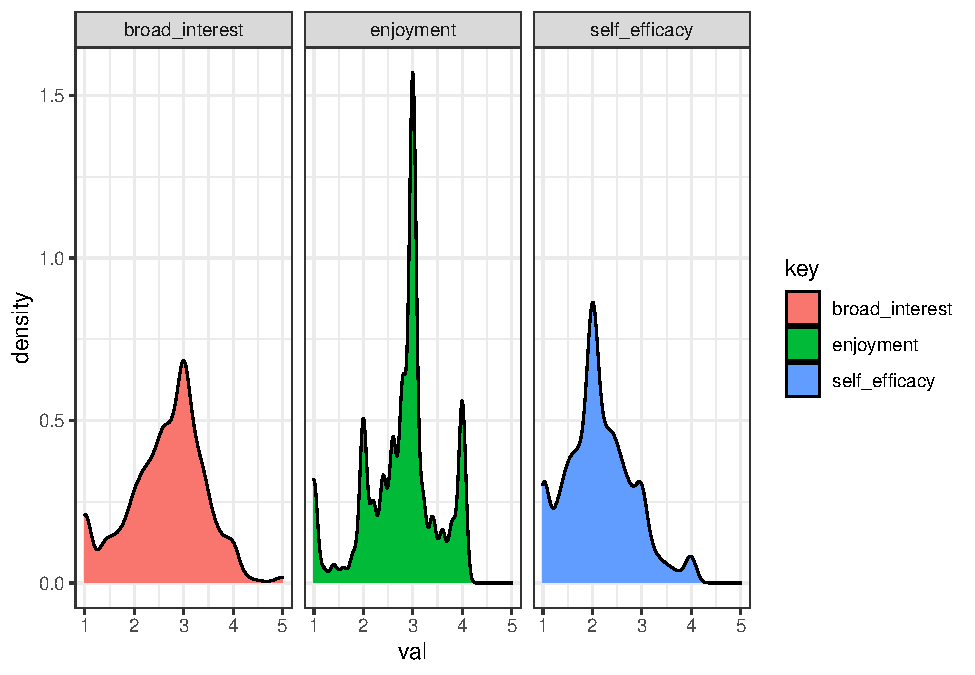
\includegraphics{paper_files/figure-latex/unnamed-chunk-7-1.pdf}

\hypertarget{model-specification}{%
\subsection{Model specification}\label{model-specification}}

In addition to the number of profiles (specified with the \texttt{n\_profiles}
argument), the model can be specified in terms of whether and how the variable
variances and covariances are estimated.

The models are specified by passing arguments to the \texttt{variance} and \texttt{covariance}
arguments. The possible values for these arguments are:

\begin{itemize}
\tightlist
\item
  \texttt{variances}: ``equal'' and ``zero''
\item
  \texttt{covariances}: ``varying'', ``equal'', and ``zero''
\end{itemize}

If no values are specified for these, then the variances are constrained to be
equal across classes, and covariances are fixed to 0 (conditional independence
of the indicators).

These arguments allow for four models to be specified:

\begin{itemize}
\tightlist
\item
  Equal variances and covariances fixed to 0 (Model 1)
\item
  Varying variances and covariances fixed to 0 (Model 2)
\item
  Equal variances and equal covariances (Model 3)
\item
  Varying variances and varying covariances (Model 6)
\end{itemize}

Two additional models (Models 4 and 5) can be fit using MPlus. More information
on the models can be found in the
\href{https://data-edu.github.io/tidyLPA/articles/Introduction_to_tidyLPA.html}{vignette}.

Here is an example of specifying a model with varying variances and covariances
(Model 6; not run here):

\hypertarget{comparing-a-wide-range-of-solutions}{%
\subsection{Comparing a wide range of solutions}\label{comparing-a-wide-range-of-solutions}}

The function \texttt{compare\_solutions()} compares the fit of several estimated models,
with varying numbers of profiles and model specifications:

\hypertarget{accessing-values-in-the-output}{%
\subsection{Accessing values in the output}\label{accessing-values-in-the-output}}

A few helper functions are available to make it easier to work with the output
of an analysis.

\texttt{get\_data()} returns the data:

\begin{verbatim}
## # A tibble: 700 x 9
##    model_number classes_number broad_interest enjoyment self_efficacy Class
##           <dbl>          <int>          <dbl>     <dbl>         <dbl> <dbl>
##  1            1              3            3.8       4            1        1
##  2            1              3            3         3            2.75     3
##  3            1              3            1.8       2.8          3.38     3
##  4            1              3            1.4       1            2.75     2
##  5            1              3            1.8       2.2          2        3
##  6            1              3            1.6       1.6          1.88     3
##  7            1              3            3         3.8          2.25     1
##  8            1              3            2.6       2.2          2        3
##  9            1              3            1         2.8          2.62     3
## 10            1              3            2.2       2            1.75     3
## # … with 690 more rows, and 3 more variables: Class_prob <int>,
## #   Probability <dbl>, id <int>
\end{verbatim}

We note that \texttt{get\_data()} returns data in wide format when applied to an object
of class tidyProfile (one element of a tidyLPA object), or when applied to a
tidyLPA object of length one. \texttt{get\_data()} returns long format when applied to a
tidyLPA object containing multiple tidyProfile analyses (because then the wide
format does not make sense).

To transform data in the wide format into the long format, the \texttt{gather()}
function from the \textbf{tidyr} package can be used, e.g.:

\begin{verbatim}
## # A tibble: 700 x 9
##    model_number classes_number broad_interest enjoyment self_efficacy Class
##           <dbl>          <int>          <dbl>     <dbl>         <dbl> <dbl>
##  1            1              3            3.8       4            1        1
##  2            1              3            3         3            2.75     3
##  3            1              3            1.8       2.8          3.38     3
##  4            1              3            1.4       1            2.75     2
##  5            1              3            1.8       2.2          2        3
##  6            1              3            1.6       1.6          1.88     3
##  7            1              3            3         3.8          2.25     1
##  8            1              3            2.6       2.2          2        3
##  9            1              3            1         2.8          2.62     3
## 10            1              3            2.2       2            1.75     3
## # … with 690 more rows, and 3 more variables: Class_prob <int>,
## #   Probability <dbl>, id <int>
\end{verbatim}

\hypertarget{recommendations-regarding-analytic-choices}{%
\section{Recommendations Regarding Analytic Choices}\label{recommendations-regarding-analytic-choices}}

\hypertarget{grolts-checklist}{%
\subsection{GRoLTs checklist}\label{grolts-checklist}}

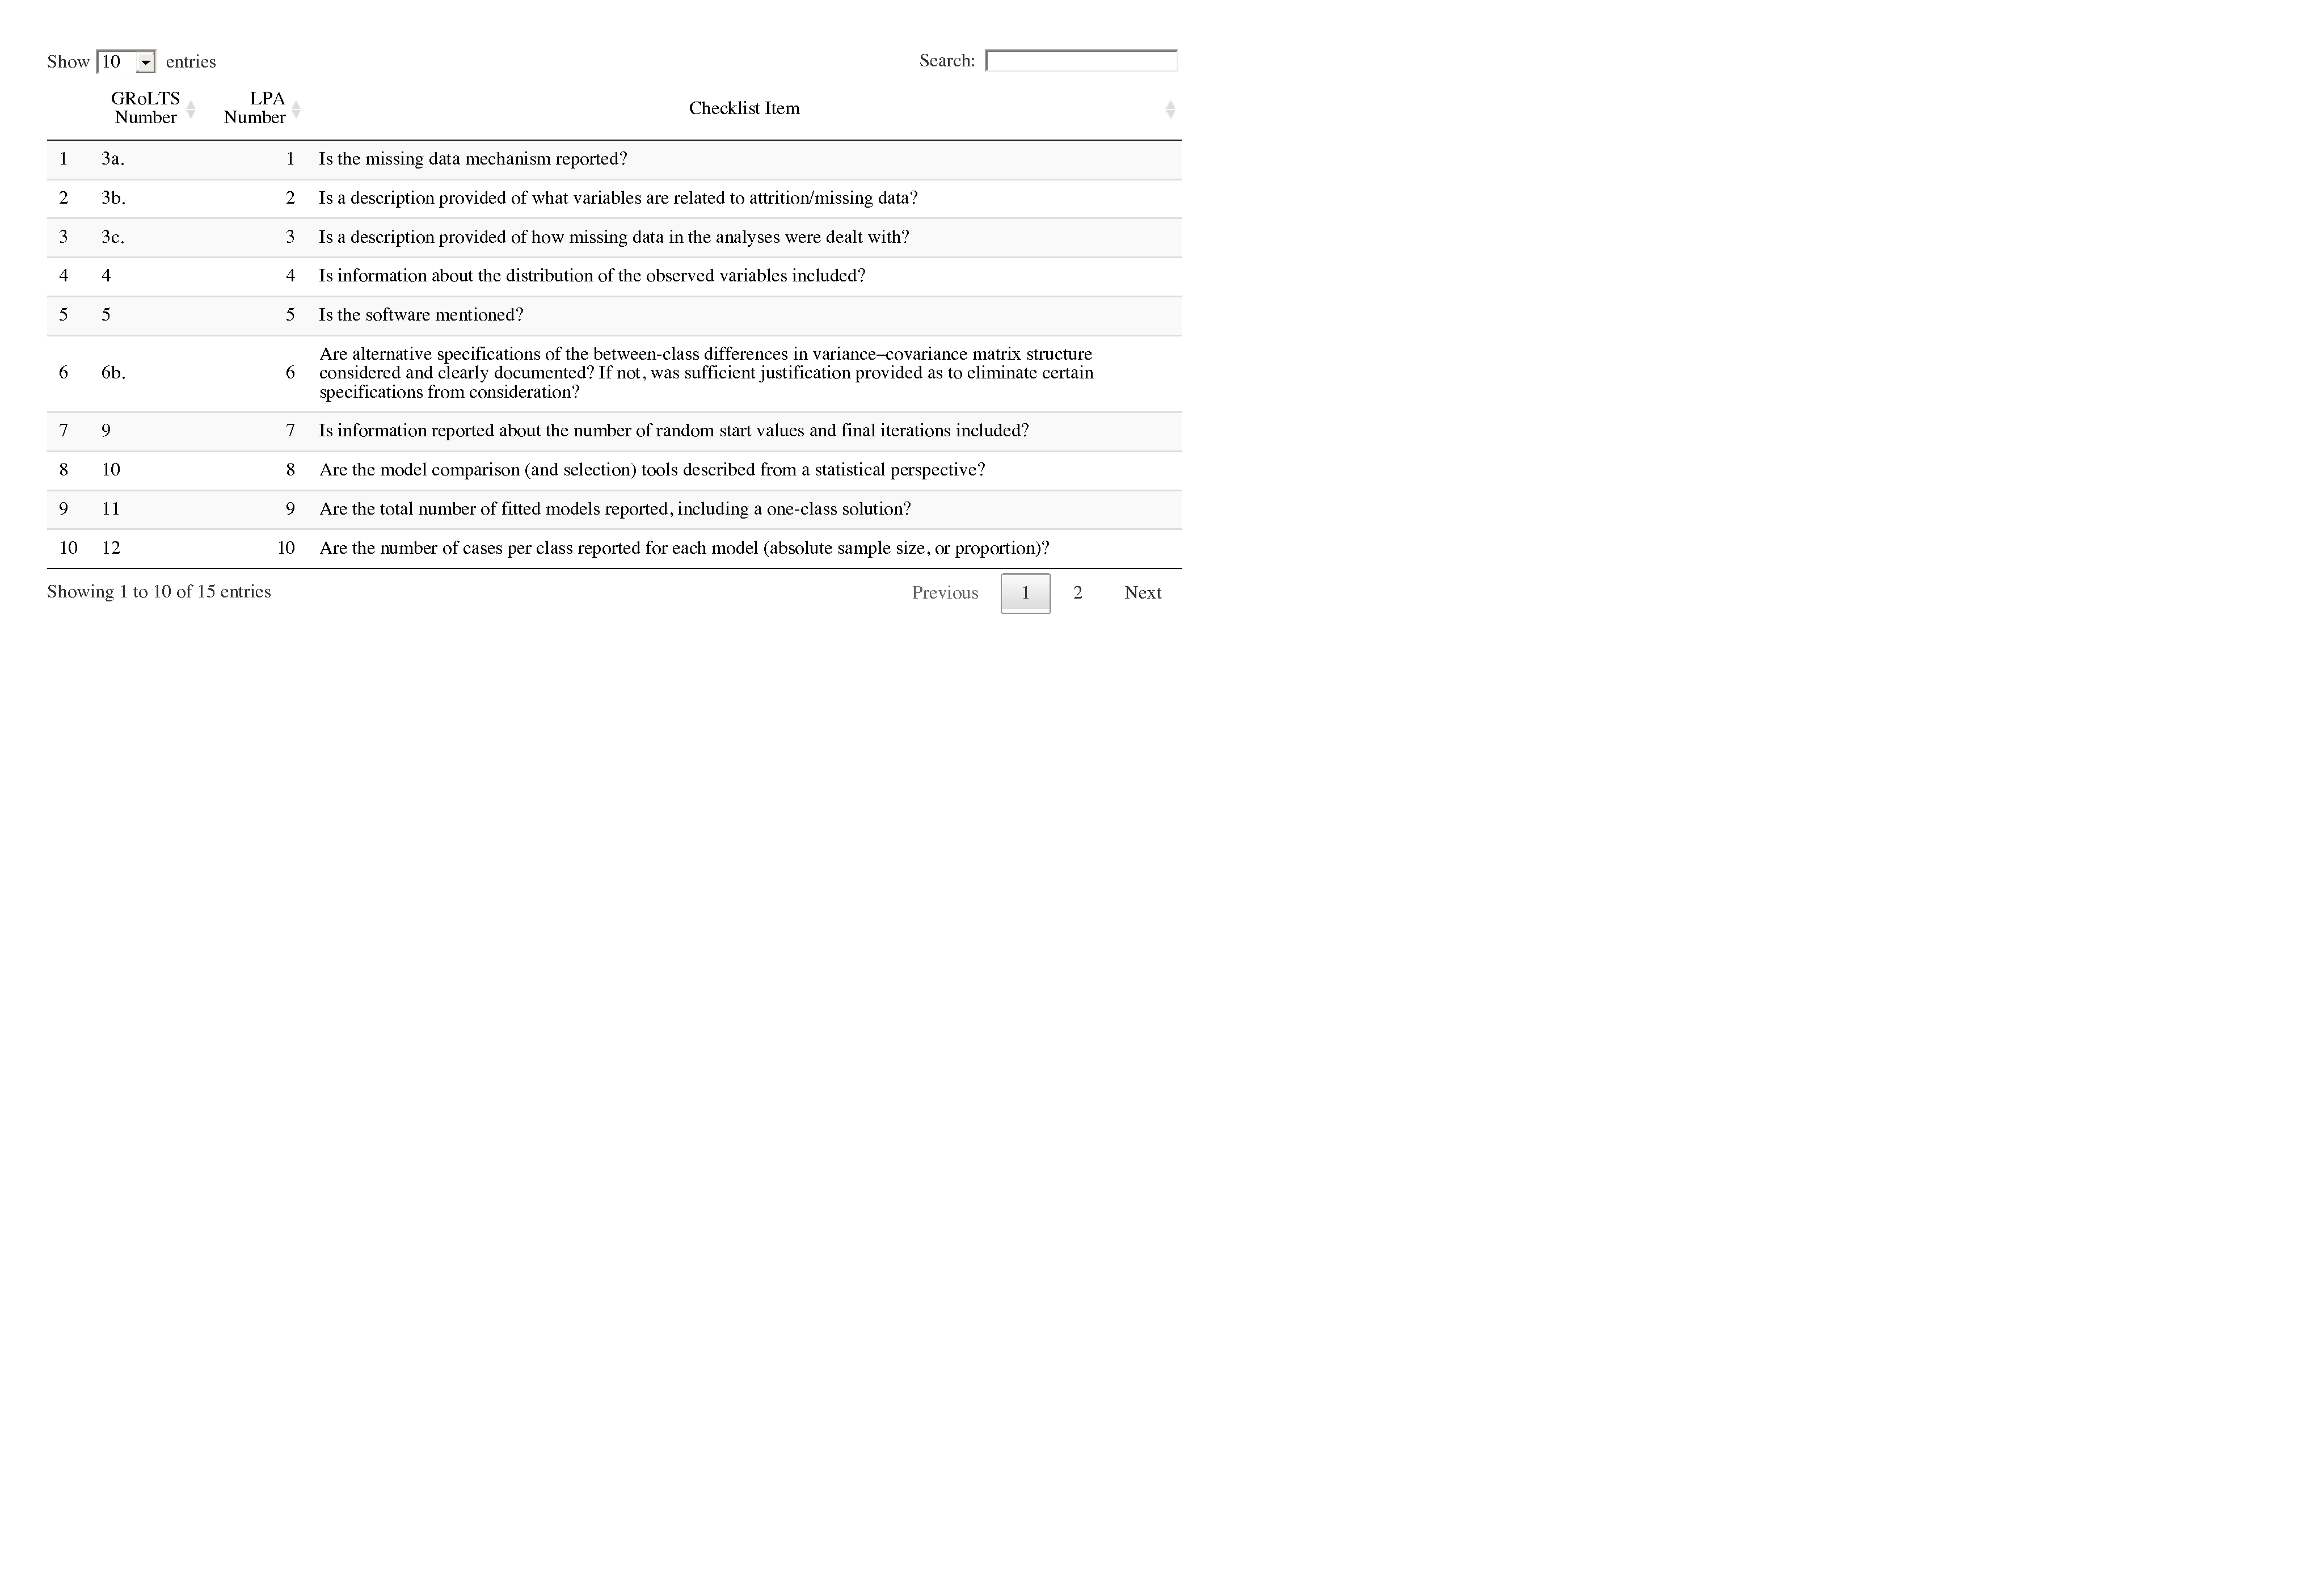
\includegraphics{paper_files/figure-latex/unnamed-chunk-13-1.pdf}

We walk through each of these in turn.

\hypertarget{is-the-missing-data-mechanism-reported}{%
\subsubsection{Is the missing data mechanism reported?}\label{is-the-missing-data-mechanism-reported}}

\hypertarget{is-a-description-provided-of-what-variables-are-related-to-attritionmissing-data}{%
\subsubsection{Is a description provided of what variables are related to attrition/missing data?}\label{is-a-description-provided-of-what-variables-are-related-to-attritionmissing-data}}

\hypertarget{is-a-description-provided-of-how-missing-data-in-the-analyses-were-dealt-with}{%
\subsubsection{Is a description provided of how missing data in the analyses were dealt with?}\label{is-a-description-provided-of-how-missing-data-in-the-analyses-were-dealt-with}}

\hypertarget{is-information-about-the-distribution-of-the-observed-variables-included}{%
\subsubsection{Is information about the distribution of the observed variables included?}\label{is-information-about-the-distribution-of-the-observed-variables-included}}

\hypertarget{is-the-software-mentioned}{%
\subsubsection{Is the software mentioned?}\label{is-the-software-mentioned}}

\hypertarget{are-alternative-specifications-of-the-between-class-differences-in-variancecovariance-matrix-structure-considered-and-clearly-documented}{%
\subsubsection{Are alternative specifications of the between-class differences in variance--covariance matrix structure considered and clearly documented?}\label{are-alternative-specifications-of-the-between-class-differences-in-variancecovariance-matrix-structure-considered-and-clearly-documented}}

\hypertarget{is-information-reported-about-the-number-of-random-start-values-and-final-iterations-included}{%
\subsubsection{Is information reported about the number of random start values and final iterations included?}\label{is-information-reported-about-the-number-of-random-start-values-and-final-iterations-included}}

\hypertarget{are-the-model-comparison-and-selection-tools-described-from-a-statistical-perspective}{%
\subsubsection{Are the model comparison (and selection) tools described from a statistical perspective?}\label{are-the-model-comparison-and-selection-tools-described-from-a-statistical-perspective}}

\hypertarget{are-the-total-number-of-fitted-models-reported-including-a-one-class-solution}{%
\subsubsection{Are the total number of fitted models reported, including a one-class solution?}\label{are-the-total-number-of-fitted-models-reported-including-a-one-class-solution}}

\hypertarget{are-the-number-of-cases-per-class-reported-for-each-model-absolute-sample-size-or-proportion}{%
\subsubsection{Are the number of cases per class reported for each model (absolute sample size, or proportion)?}\label{are-the-number-of-cases-per-class-reported-for-each-model-absolute-sample-size-or-proportion}}

\hypertarget{if-classification-of-cases-in-a-trajectory-is-the-goal-is-entropy-reported}{%
\subsubsection{If classification of cases in a trajectory is the goal, is entropy reported?}\label{if-classification-of-cases-in-a-trajectory-is-the-goal-is-entropy-reported}}

\hypertarget{are-all-of-the-estimates-plotted}{%
\subsubsection{Are all of the estimates plotted?}\label{are-all-of-the-estimates-plotted}}

\hypertarget{are-the-raw-data-plotted-along-with-the-estimates}{%
\subsubsection{Are the raw data plotted along with the estimates?}\label{are-the-raw-data-plotted-along-with-the-estimates}}

\hypertarget{are-characteristics-of-the-final-class-solution-numerically-described-i.e.-means-sdse-n-ci-etc.}{%
\subsubsection{Are characteristics of the final class solution numerically described (i.e., means, SD/SE, n, CI, etc.)?}\label{are-characteristics-of-the-final-class-solution-numerically-described-i.e.-means-sdse-n-ci-etc.}}

\hypertarget{are-the-syntax-files-available-either-in-the-appendix-supplementary-materials-or-from-the-authors}{%
\subsubsection{Are the syntax files available (either in the appendix, supplementary materials, or from the authors)?}\label{are-the-syntax-files-available-either-in-the-appendix-supplementary-materials-or-from-the-authors}}

There are a number of analytic choices that need to be made when carrying out
person-oriented analyses. Because such person-oriented approaches are often more
subjective (in practice) than other approaches (Linnenbrink-Garcia and
Wormington, 2017), there is no one rule for determining the solution obtained.
This solution is obtained on the basis of multiple decisions, such as the number
of profiles selected or the modeling decisions such as what specific options are
used for the cluster analysis (i.e., the distance metric used to calculate the
similarity of the observations as part of the Ward's hierarchical clustering) or
what parameters are estimated and how as part of LPA.

Given the subjectivity involved, it is important that researchers be transparent
and work as part of a team to obtain clustering solutions. Transparency about
the design and analytic choices is important so that readers can appropriately
interpret the report. Researchers can enhance transparency and reproducibility
by sharing detailed descriptions of methodology and document it through the use
of syntax (and, if possible, data) that we share with others. Working as part of
a team can help to serve as a check on several of the choices researchers make,
such as over-fitting or under-fitting the model to the data. Each decision
depends on multiple factors and balancing tensions. We discuss each of the key
decisions listed in an analysis.

\hypertarget{how-the-data-are-centering-or-scaled}{%
\subsection{How the Data are Centering or Scaled}\label{how-the-data-are-centering-or-scaled}}

The data can be transformed by centering or scaling. Typically, these are done
after the profiles are created, so that differences between profiles can be more
easily explored. They can also be done prior to the analysis, which can be
helpful for obtaining solutions when the variables are on very different
scales.

\hypertarget{how-to-choose-the-number-of-profilesclasses}{%
\subsection{How to Choose the Number of Profiles/Classes}\label{how-to-choose-the-number-of-profilesclasses}}

In the case of choosing the number of profiles (and the specification of the
model / profile solution), multiple criteria, such as the BIC or the proportion
of variance explained are recommended for decision-making, but also
interpretability in light of theory, parsimony, and evidence from
cross-validation should be considered.

\hypertarget{how-to-choose-options-for-the-clustering-procedure-or-to-select-the-model-parameterization}{%
\subsection{How to Choose Options for the Clustering Procedure or to Select the Model Parameterization}\label{how-to-choose-options-for-the-clustering-procedure-or-to-select-the-model-parameterization}}

In LPA, we can determine which parameters - variance
and covariance - are estimated to be the same or different across all profiles,
and, in the case of covariance, whether it is fixed to zero. Of course, for the
profiles we are most interested in, the mean is allowed to vary across profiles.
The models with more parameters freely-estimated use more degrees of freedom;
thus, similar to the number of profiles selected, the balance between adding
more parameters (and having a more complex model) and interpretability and
parsimony must be balanced. If a more complex model fits better and is
interpretable and is justifiable in terms of the data collected, then it may be
preferred to simpler models. If the two models are similar in terms of their
fit, then the more simple, parsimonious model should be selected.

\hypertarget{more-general-recommendations}{%
\subsection{More General Recommendations}\label{more-general-recommendations}}

This section highlights three general recommendations. First, scholars taking a
person-oriented approach should emphasize reproducibility in carrying out
analyses. This is in part due to the exploratory and interpretative nature of
person-oriented approaches. To this end, presenting multiple models, as in
Pastor et al. (2007), should be encouraged, rather than presenting one solution.
In addition, having multiple analysts review the solutions found is encouraged.
As part of this recommendation, we suggest that researchers consider how their
analyses can be reproduced by other analysts outside of the research team:
Sharing code and data is an important part of this work. Also related,
researchers should consider how profiles are replicated across samples.

A second general recommendation considers more flexibly incorporating time, when
data are collected across multiple time points, into analyses. ISOA groups all
time points and doesn't make distinctions. Other approaches perform analysis
separately at different timepoints (Corpus \& Wormington, 2014). Some integrate
time as a part of the profiles, i.e.~growth mixture modeling (groups of
patterns), i.e.~within-person growth modeling, where there are individual growth
patterns. Research to date has yet to consider additional challenges in applying
person centered approaches to longitudinal data. For instance, Schmidt et al
(2018) use an Experience Sampling Method (ESM) approach to collecting data and
used a person-centered approach to generate profiles of students in science
class. This work does not account for student-level effects. In other words, it
did not model the shared variance of multiple observations of the same student.

Third, best practices in within-person or longitudinal research call for
modeling the nesting structure. However, researchers have yet to successfully
incorporate this practice into the person centered approach. One way to approach
this is to use cross-classified mixed effects models, as in Strati, Schmidt, and
Maier (2017) and in Rosenberg (2018). In such approaches, dependencies in terms
of, for example, individuals responding to (ESM) surveys at the same time and
repeated responses being associated with the same individuals can both be
modeled, although the effects of these two sources of dependencies are not
nested as in very common uses of multi-level models, but rather are
cross-classified. West, Welch, \& Galecki (2014) have a description of the use of
multi-level models with cross-classified data and tools (including those freely
available through R) that can be used to estimate them.

\hypertarget{conclusion}{%
\section{Conclusion}\label{conclusion}}

Person-oriented analysis ia way to consider how psychological constructs are
experienced (and can be analyzed) together and at once. Though described in
contrast to a variable-centered approach, scholars have pointed out how
person-oriented approaches are complementary to variable-centered analyses
(Marsh, Ludtke, Trautwein, \& Morin, 2009). A person-oriented approach can help
us to consider multiple variables together and at once and in a more dynamic
way, reflected in the methodological approaches for cluster analysis and LPA
that identify profiles of individuals responses.

This manuscript provided an outline of how to get started with person-oriented
analyses in an informed way. We provided a general overview of the methodology
and described tools to carry out such an analysis. We also described specific
tools, emphasizing freely-available open-source options that we have developed.
Because of the inherently exploratory nature of person-oriented analysis,
carrying out the analysis in a trustworthy and open way is particularly
important. In this way, the interpretative aspect of settling on a solution
shares some features of quantitative and qualitative research: The systematic
nature of quantitative research methods (focused upon agreed-upon criteria such
as likelihood-ratio tests) and qualitative research methods (focused upon the
trustworthiness of both the analysis and the analyst) are important to consider
when carrying out person-oriented analysis. Lastly, we made some general
recommendations for future directions--and also highlighted some situations for
which person-oriented approaches may not be the best and some cautions raised in
past research regarding how such approaches are used.

In conclusion, as use of person-oriented approaches expand, new questions and
opportunities for carrying out research in a more holistic, dynamic way will be
presented. Analyzing constructs together and at once is appealing to
researchers, particularly those carrying out research in fields such as
education for which communicating findings to stakeholders in a way that has the
chance to impact practice is important. Our aim was not to suggest that such an
approach is always the goal or should always be carried out, but rather to
describe how researchers may get started in an informed way as researchers seek
to understand how individuals interact, behave, and learn in ways that embraces
the complexity of these experiences.

\newpage

\hypertarget{references}{%
\section{References}\label{references}}

\begingroup
\setlength{\parindent}{-0.5in}
\setlength{\leftskip}{0.5in}

\hypertarget{refs}{}
\leavevmode\hypertarget{ref-R-tidyLPA}{}%
Rosenberg, J. M., Beymer, P. N., Anderson, D. J., Lissa, C. van, \& Schmidt, J. A. (2018). TidyLPA: An r package to easily carry out latent profile analysis (lpa) using open-source or commercial software. \emph{Journal of Open Source Software}, \emph{3}(30), 978. doi:\href{https://doi.org/10.21105/joss.00978}{10.21105/joss.00978}

\endgroup

\end{document}
